\documentclass[sigconf]{acmart}

% \renewcommand\footnotetextcopyrightpermission[1]{} % removes footnote with conference information in first column
\pagestyle{fancy} % removes running headers
\usepackage{booktabs} % For formal tables

\usepackage{url}
\usepackage{algorithm}
\usepackage[noend]{algpseudocode}
\algtext*{EndWhile}% Remove "end while" text
\algtext*{EndIf}% Remove "end if" text
%\usepackage{flexisym}

\setlength{\parskip}{0pt}
\setlength{\parsep}{0pt}
\setlength{\headsep}{0pt}
\setlength{\topskip}{0pt}
\setlength{\topmargin}{0pt}
\setlength{\topsep}{0pt}
\setlength{\partopsep}{0pt}
%\linespread{0.95}
\usepackage{mdwlist}

\usepackage{amsmath}
\fancyhead{}
\settopmatter{printacmref=false, printfolios=false}
% Copyright
\setcopyright{none}
% \setcopyright{acmcopyright}
% \setcopyright{acmlicensed}
% \setcopyright{rightsretained}
% \setcopyright{usgov}
% \setcopyright{usgovmixed}
% \setcopyright{cagov}
% \setcopyright{cagovmixed}

\settopmatter{printacmref=false} % Removes citation information below abstract
\begin{document}
\title{\textit{Sample*} Diachronically Like-minded User Community Detection}\titlenote{Link to Github or an online repo}
\author{Ali Fani}
% \authornote{Laboratory for Systems, Software and Semantics (LS$^3$)}
%\orcid{1234-5678-9012}
\affiliation{
  \institution{University of Windsor}
%   \streetaddress{P.O. Box 1212}
%   \city{Toronto} 
%   \state{ON} 
%   \country{Canada} 
%   \postcode{43017-6221}
}
\email{afani@uwindsor.ca}
\author{Hossein Fani}
% \authornotemark[1]
\orcid{0000-0002-6033-6564}
\affiliation{
 \institution{University of Windsor}
%   \city{Fredericton} 
%   \state{NB} 
%   \country{Canada} 
}\email{hfani@uwindsor.ca}

\maketitle
\section{Experimental Setup and Evaluation}\label{experiment}
%This section describes the experiments performed to validate our proposed work in comparison with two baselines in the context of news recommendation, user prediction, and community selection applications on a Twitter dataset.

\subsection{Dataset}
In our experiments, we use a publicly available Twitter dataset collected and published\footnote{\href{http://www.wis.ewi.tudelft.nl/umap2011/}{www.wis.ewi.tudelft.nl/umap2011/}} by Abel et al.~\cite{DBLP:conf/um/AbelGHT11}. It consists of approximately 3M tweets posted by 135,731 unique users between November 1 and December 31, 2010. In addition to its text, each tweet includes user id and timestamp. The whole two months time period is sampled on a daily basis, i.e., L = 61 days.

\subsection{Setup}
Our proposed approach consists of three phases to identify temporally like-minded user communities; finding topics, building user vector representations, and detecting user communities. Here, we provide the implementation details and the setup of our approach in each of these phases. 


\subsubsection{Finding topics}
Extracting topics from tweets suffers from the sparsity problem when topic modeling methods such as LDA are used~\cite{escri/ZarrinkalamB17}. As suggested in~\cite{DBLP:conf/ecir/ZarrinkalamFBK17, DBLP:conf/ecir/ZarrinkalamFBK16}, we annotate each tweet with entities defined in Wikipedia to obtain better topics from Twitter with no change in the underlying topic detection methods. For instance, for a tweet such as `\textit{NATO Leaders Seek Time on Afghan Exit Strategy - \href{http://nyti.ms/cMMDuR}{http://nyti.ms/cMMDuR}}', a semantic annotator such as TagMe~\cite{DBLP:conf/cikm/FerraginaS10} is able to identify and extract several Wikipedia entities, namely `\href{https://en.wikipedia.org/wiki/NATO}{NATO}'\footnote{\href{https://en.wikipedia.org/wiki/NATO}{en.wikipedia.org/wiki/NATO}}, `\href{https://en.wikipedia.org/wiki/Afghanistan}{Afghan}', and `\href{https://en.wikipedia.org/wiki/Exit_strategy}{Exit\_Strategy}'. Using entities instead of words can lead to the reduction of noisy content within the topic detection process, because each concept implicitly represents a collection of typical terms which are collectively more meaningful than a single word or a group of less coherent words~\cite{DBLP:conf/wims/PetkosPASK14}. We annotated the text of each tweet with Wikipedia entities using the TAGME RESTful API\footnote{\href{https://services.d4science.org/web/tagme/documentation}{services.d4science.org/web/tagme/documentation}}, which resulted in 350,731 unique entities. 

In order to find topics of interest in our dataset, we have applied MALLET\footnote{\href{http://mallet.cs.umass.edu/topics.php}{mallet.cs.umass.edu/topics.php}} for LDA. LDA-based approaches to topic detection need \textit{a priori} knowledge for the number of topics. The number of topics has been already investigated and set to 50 for the same tweet dataset by other researchers in~\cite{DBLP:journals/ci/FaniBZZD17}. We populate the points of temporal interest (PoTI) for our topic set $\mathbb{Z}$ on a daily basis, i.e., L = 61 days, and screen out values less than 0.1. The condition for homogeneity $c$ is set such that the difference of values falls in the range $[0, 0.1)$.

\subsubsection{Building user vector representation}
We extended CBOW architecture in Gensim\footnote{\href{https://radimrehurek.com/gensim/models/word2vec.html}{radimrehurek.com/gensim/models/word2vec.html}} to learn user embeddings as already introduced in this paper. The training phase uses a learning rate of 0.025 and in each epoch we decrease it by 0.002 for 200 epochs. We perform the experiments on different vector sizes of $d={100,200,...,500}$ in an increasing order till we see no further performance gain.

\subsubsection{Detecting user communities}
We build temporal topic-based communities according to our proposed approach in Section \ref{community_detection}. We build the weighted graph G and apply the Louvain method with resolution parameter 0.1 using Pajek\footnote{\href{http://vlado.fmf.uni-lj.si/pub/networks/pajek/}{vlado.fmf.uni-lj.si/pub/networks/pajek/}}. This leads to our temporal topic-based communities $\mathbb{P}^*$. 

\subsection{Baselines}
We compare our work against the following baselines whose details has been already given in the related work section: 

\textbf{Fani et al.~\cite{DBLP:journals/ci/FaniBZZD17}}. This approach models user's contributions toward the topics of interest through a multivariate time series. We use LDA in its topic detection step with 50 topics and build the time series for daily time intervals L= 61 days in its user modeling step. The approach uses two dimensional cross correlation to measure the similarity of a pair of users' time series. We use the implementation in MATLAB\footnote{\href{https://www.mathworks.com/help/signal/ref/xcorr2.html}{www.mathworks.com/help/signal/ref/xcorr2.html}} for calculating time series cross-correlation. Finally, we use the Louvain method in Pajek for its community detection step as proposed by the authors. 

\textbf{Hu et al.~\cite{DBLP:conf/aaai/HuYC14}} . This is a parametric unified probabilistic generative model for topics and communities. The number of topics is set to 50 and we perform experiments on increasing number of communities for $C={5,10,...,30}$ till we see no performance gain. The number of iterations is set to 1,000. This method is a mixture model in which all users are members of all communities with a probability distribution. In our comparison, we only consider the community with the highest probability as each user's community.


Figure \ref{user_distribution_stacked} provides an overview of the distribution of users across different communities. For Hu et al.'s work, the number of communities needs to be specified as shown ranging from 5 to 30. For our proposed approach, the number of communities is automatically determined by the graph partitioning method; however, the size of the embeddings needs to be provided, which has been set from 100 to 500. As seen in the figure, our proposed method leads to a more fair distribution of users across communities while the two baseline methods have a higher skewness in the distribution of users in their identified communities. While this by itself is not a measure of community quality, as we will show later, disproportionate distribution of users in communities could lead to poor application level performance.

\subsection{Evaluation Protocol and Gold Standard}
On the one hand, contrary to typically small scale networks or synthetic ones, gold standard communities for real social networks are not available. So, well-defined quality measures such as Rand index, Jaccard index, or normalized mutual information (NMI) that require comparison to a gold standard are not applicable. On the other hand and in the absence of a golden standard, quality functions such as \textit{modularity} are not helpful either since they are based on the explicit links between users, which are not applicable to our work. For instance, in the context of our work and the baselines, a perfect community detection algorithm might have a low modularity value as those users that are deemed most similar might not have explicit social connection with each other. Therefore in our work, the communities that achieve high modularity are not necessarily optimal from temporal and topical points of view ~\cite{Moradi2012}. 

Fortunately, the performance of community detection methods can be measured through observations made at the application level, as suggested in~\cite{DBLP:conf/sigmod/HuYCX15, Moradi2012}. In these evaluation strategies, a temporal like-minded user community detection method is considered better iff its output communities improve an underlying application. We deploy three applications: news recommendation, user prediction, and community selection. Note should be taken that we do not attempt to improve the state of the art in any of these three applications but rather to show that the application of the proposed community detection method is able to provide a stronger performance compared to the other two state of the art community detection baselines. 

To this end, we first build a gold standard dataset for the said applications by collecting news articles to which a user has explicitly linked in her tweets (or retweets). We postulate that users post news article urls since they are interested in the topics of those news articles. Similar to tweets, we annotate news articles with Wikipedia entities. We build the gold standard from a set of news articles whose urls have been posted by user $u$ at time $t$. We see each entry as a triple $(u, a, t)$ consisting of the news article $a$, user $u$, and the time $t$. As a result, $\mathbb{G}=\{(u,a,t): u\in\mathbb{U},a\in\mathbb{A},1\leq{t}\leq{L=61}\}$ forms our gold standard where $\mathbb{U}$ and $\mathbb{A}$ are sets of users and news articles. The gold standard $\mathbb{G}$ consists of 25,756 triples extracted from 3,468 distinct news articles posted by 1,922 users.

\begin{figure}[t]
\centering
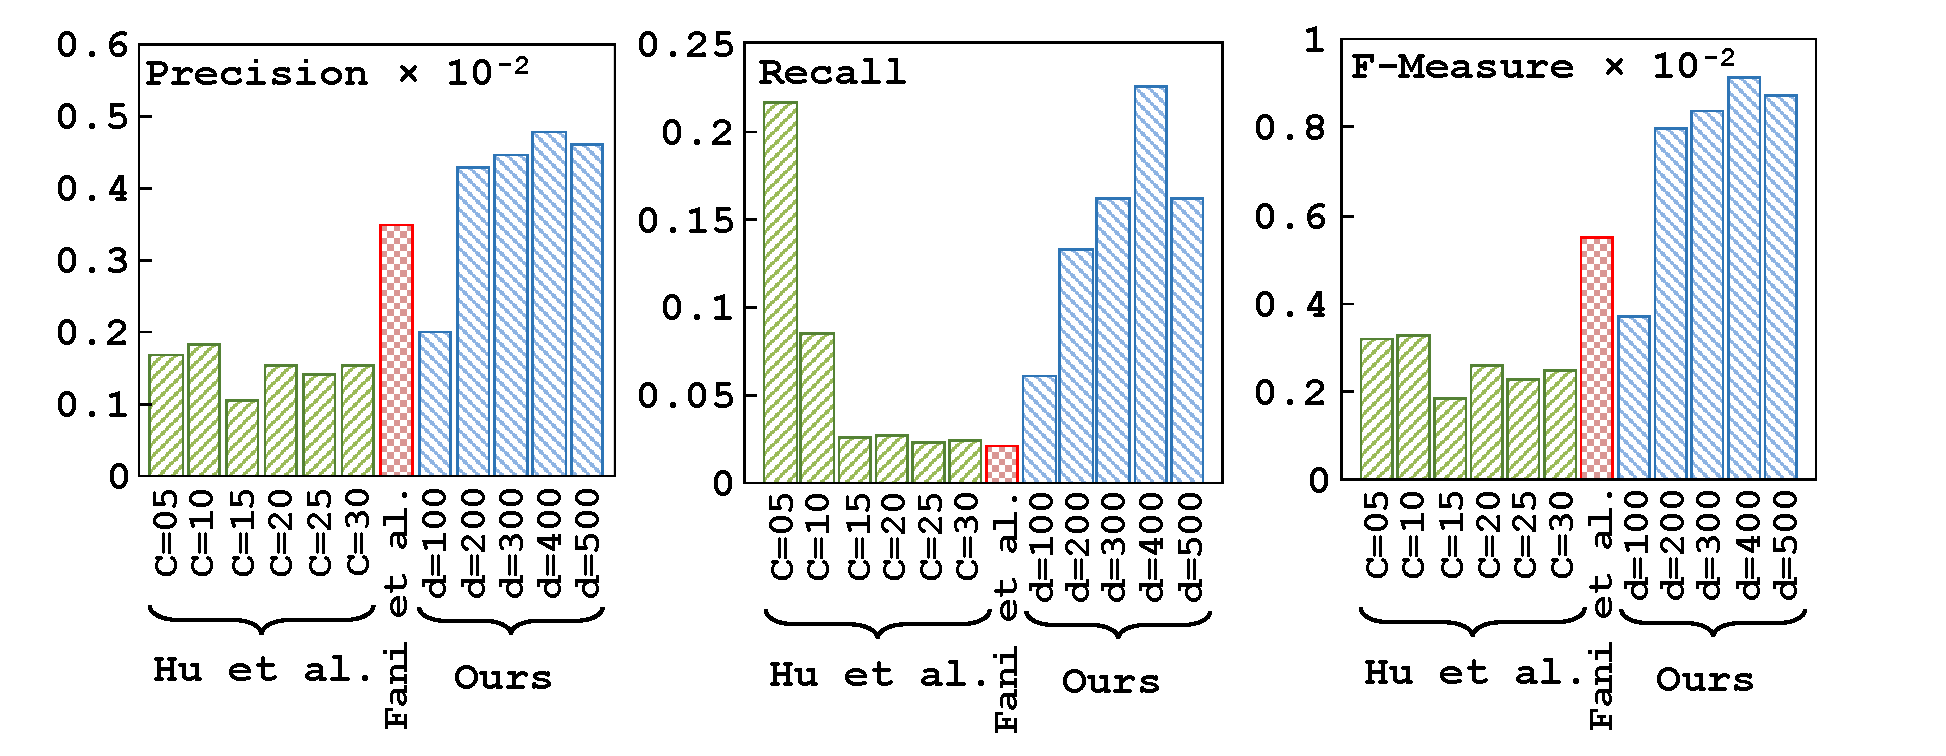
\includegraphics[width=1.05\columnwidth]{Images/user_prediction.eps}
\caption{Comparative performance on the user prediction application.}\label{user_prediction}
\end{figure}

\subsection{User Prediction}
Another application with which we evaluate our approach and the baselines is the user prediction application. Given the gold standard $\mathbb{G}$ and the like-minded user communities $\mathbb{P}^*$, this time the goal is to predict which users posted the news article $a$ at time $t$. To do so, we find the closest community to the news article in terms of topics of interest at time $t$. Then, the members of such community would constitute our prediction list. We employ precision, recall, and f-measure to report user prediction performance. We summarize the results for these metrics in Figure \ref{user_prediction}. As shown, in terms of precision, our approach with all different dimensions except $d=100$ outperforms all other baselines. In terms of recall, however, Hu et al.~\cite{DBLP:conf/aaai/HuYC14} with $C=5$ competes with our proposed approach when $d=400$. The reason for such high recall in Hu et al. with C=5 can be attributed to the lower number of communities in this method. The fewer the number of communities are, the higher the recall of the method would be. In other words, if we only have one community that includes all users, recall would be 1.0. As the number of communities increases from $C=10$ to $C=30$ in Hu et al, recall decreases which supports our explanation. Overall, F-measure shows the superiority of approach in user prediction in all its variants except for $d=100$, which is weaker than Fani et al. 
\begin{figure}[t]
\centering
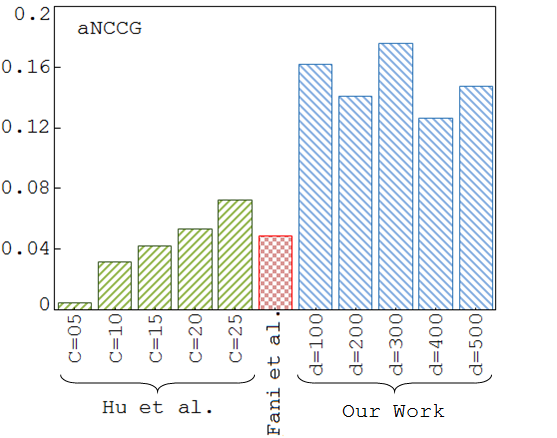
\includegraphics[width=.6\columnwidth]{Images/community_selection.png}
\caption{Performance on community selection application.\label{community_selection}}
\end{figure}
\subsection{Community Selection}
In the realm of cluster-based information retrieval systems, the entire collection of documents are split into clusters such that only the documents in highly related clusters to a given query are accessed. As a result, fewer documents are searched from within a large collection of documents which results in improved response time. Better clustering solutions in this context are those that can group relevant documents for previously unseen queries. This approach is referred to as \textit{collection selection} and normalised cumulative cluster gain (NCCG) \cite{DBLP:conf/inex/NayakVKGDG09} is a metric used for evaluating collection selection. According to NCCG, the best clustering would be the one where all the documents related to a given query are all located in the same cluster. The worst clustering is the one where the relevant documents to an input query are scattered across many clusters. NCCG is the difference between the current clustering gain and the worst possible, formulated as follows:
\begin{equation}
NCCG=\frac{s-s_{min}}{1-s_{min}}    
\end{equation}
where $s=\frac{\sum\limits^{|g|}{cumsum(g)}}{n^2}$ and $g$ is a sorted gain vector whose elements represent each cluster's gain, i.e., the number of relevant documents in a cluster, $n$ is the total number of relevant documents and $cumsum$ represents the cumulative sum of a vector. The worst possible gain $s_{min}$ happens when the relevant documents to the query are uniformly distributed over all clusters. 

However, NCCG has been criticized for being sensitive to the number of clusters and population distribution; therefore, De Vries et al. \cite{DBLP:journals/corr/abs-1208-5654} have proposed an \textit{adjusted} version of NCCG (aNCCG), i.e., NCCG's divergence from a random null base model, to alleviate such problem. We employ aNCCG to evaluate the temporal and topical coherence of the identified output communities of the different approaches in the application of community selection as follows: given a news article $a$ at time $t$ (the input query), we want to find the communities of those users (similar to documents related to an input query) who have mentioned the news article at that time. The output user communities are more effective iff users who mention a news article $a$ (topical) at time $t$ (temporal) are all located in one community instead of being distributed across several communities. We report aNCCG for our approach and the baselines in Figure \ref{community_selection}. 

As seen in the figure, our approach, for different number of dimensions, outperforms the other two baselines in terms of aNCCG. This means that, in our approach, the users who mention the same news articles in specific time intervals are placed within similar user communities, i.e., such users are distributed across fewer communities. A lower aNCCG value as exhibited by Hu et al. and Fani et al. means that these methods distribute users that have posted similar news articles at specific time intervals across a larger number of user communities, which is not desirable.

\bibliographystyle{ACM-Reference-Format}
\bibliography{bibliography.bib} 

\end{document}